Model uczenia maszynowego jaki został wykorzystany w testach to sieć neuronowa.

Do testów stworzone zostało kilka modeli sieci neuronowych,
wytrenowanych na rysunkach grafów stworzonych za pomocą skryptów R.
Implementacja została wykonana biblioteką TensorFlow oraz Keras w języku Python.
Modele są w stanie rozpoznawać rysunki grafów i przypisywać im odpowiednie klasy.
Celem było również przetestowanie modeli na rzeczywistych zdjęciach,
zawierających wzorce przypominające grafy, bądź rysunkach grafów narysowanych ręcznie.

Klasy, których rozpoznawania uczony był model:
\begin{itemize}[label=-,labelsep=0.4cm,leftmargin=0.6cm]
	\item Graf bezkrawędziowy
	\item Graf pełny
	\item Drzewo binarne
	\item Ścieżka
	\item Cykl
\end{itemize}

Stworzone zostały 4 modele:
\begin{itemize}[label=-,labelsep=0.4cm,leftmargin=0.6cm]
	\item wytrenowany na danych ze stałą liczbą wierzchołków
	\item wytrenowany na danych ze stałą liczbą wierzchołków oraz walidacją krzyżową
	\item wytrenowany na danych ze zmienną liczbą wierzchołków
	\item wytrenowany na danych ze zmienną liczbą wierzchołków oraz walidacją krzyżową
\end{itemize}

\subsection{Generacja danych}
\begin{figure}[ht]
	\centering
	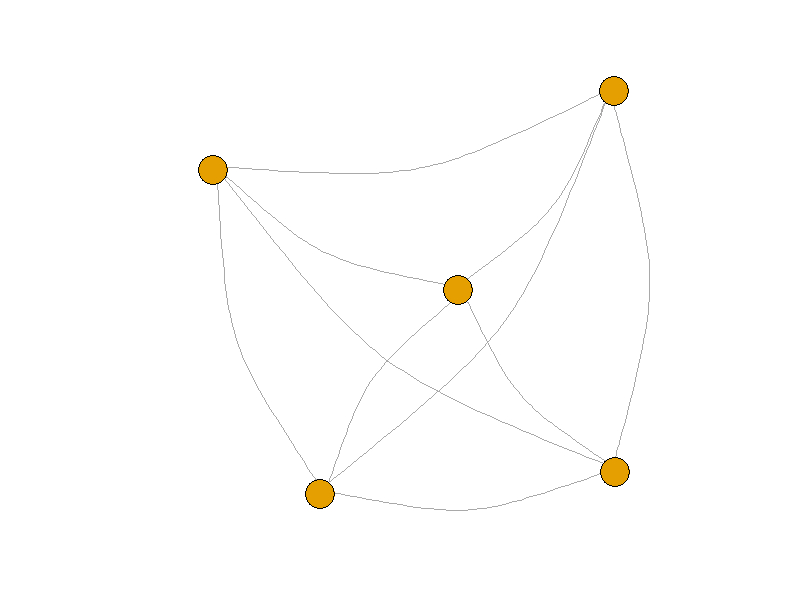
\includegraphics[height=6cm]{partials/tests/images/gen-graph_full.png}
	\caption{Przykładowy wygenerowany graf pełny}
	\label{Fig:tests-generation-1}
\end{figure}
\FloatBarrier

Dane wygenerowane zostały przy pomocy skryptu stworzonego w języku R oraz biblioteki igraph.
Skrypt został zaprojektowany funkcyjnie, by osiągnąć możliwie największą automatyzację testów.
Rysunki grafów tworzone są o wielkości 800x600 pikseli, na białym tle, z wierzchołkami w kolorze pomarańczowym,
bez jakichkolwiek oznaczeń wierzchołków oraz zapisywane są w odpowiednich katalogach, odpowiadających klasie grafu.
Przygotowane zostały funkcje tworzące ścieżki, cykle, grafy pełne, grafy bezkrawędziowe oraz drzewa binarne.
W każdej z funkcji możliwy jest wybór liczby generowanych grafów, liczba wierzchołków grafu
oraz współczynnik odpowiadający za zakrzywienie krawędzi na rysunkach.

\begin{lstlisting}[language=R,caption=Listing skryptu rysującego grafy,label={tests-generation-1}]
	#' Rysuj graf
	#'
	#' @param graph Graph - Graf do narysowania
	#' @param pathName string - Sciezka
	#' @param fileName string - Nazwa pliku
	#' @param vertexNo int - liczba wierzcholkow
	#' @param i int - Numer iteracji
	#' @param plotCurve float
	#' @return void
	#'
	plotGraphHelper <- function(graph, pathName, fileName, vertexNo, i, plotCurve)
	{
	  png(file.path(pathName, paste0(fileName, "-", vertexNo, "-", i, ".png")), width = 800, height = 600)
	  plot(graph, vertex.label = NA, edge.curved = plotCurve)
	  dev.off()
	}
\end{lstlisting}

\begin{lstlisting}[language=R,caption=Listing funkcji tworzącej ścieżkę,label={tests-generation-2}]
	#' Graf sciezka N wierzcholkow, nieskierowany
	#'
	#' @param N int - liczba rysunkow
	#' @param vertexNo int - liczba wierzcholkow
	#' @param plotCurve float
	#' @return void
	#'
	plotPaths <- function(N, vertexNo, plotCurve)
	{
		fileName <- 'path'
		pathName <- createDir(vertexNo, fileName)
		definition <- c()
		for (index in 1:(vertexNo-1))
		{
			definition <- c(definition, index, index + 1)
		}
		definitionMatrix <- matrix(definition, ncol = 2, byrow = TRUE)
		
		for (i in 1:N)
		{
			graph <- graph_from_edgelist(definitionMatrix, directed = FALSE)
			E(graph)$weight <- runif(ecount(graph))
			plotGraphHelper(graph, pathName, fileName, vertexNo, i, plotCurve)
		}
	}
\end{lstlisting}

W testach wykorzystane zostały wszystkie wybrane typy grafów.
Każdy z nich, czyli dana liczba wierzchołków i typ grafu, wygenerowany został w liczbie 500 sztuk
oraz ze stałą krzywizną krawędzi, wynoszącą 0,3.

\subsection{Dane zewnętrzne}
Obrazy testowe, które nazwane są tutaj danymi zewnętrznymi, są rysunkami grafów pochodzącymi spoza przygotowanego testu.
Dzielą się na obrazy pobrane z internetu, obrazy wygenerowane przez skrypt w R, ale nie używane w treningu,
oraz rysunki odręczne grafów. Typy danych zewnętrznych wybiegają poza klasy grafów wykorzystywanych przy uczeniu modelu.

\begin{figure}[ht]
	\centering
	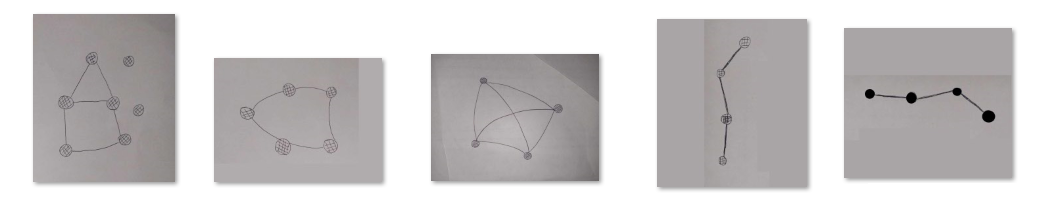
\includegraphics[width=15.5cm]{resources/tests/images/ext-graphs-drawn.png}
	\caption{Przykładowe zewnętrzne rysunki grafów narysowane odręcznie}
	\label{Fig:tests-outside-1}
\end{figure}
\FloatBarrier

\begin{figure}[ht]
	\centering
	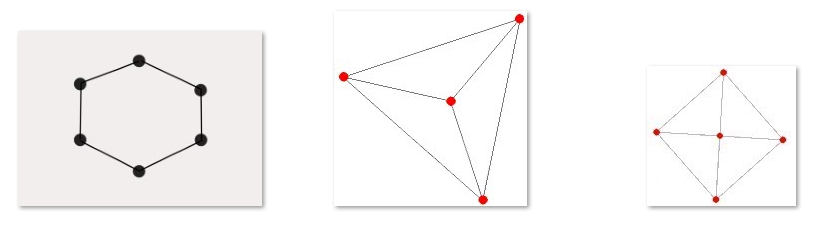
\includegraphics[width=15cm]{resources/tests/images/ext-graphs-internet.png}
	\caption{Przykładowy zewnętrzne rysunki grafów pobrane z internetu}
	\label{Fig:tests-outside-2}
\end{figure}
\FloatBarrier

\subsection{Opis ogólny skryptu}
\subsubsection{Przygotowanie}
Wszystkie przygotowane skrypty testowe rozpoczynają się od przygotowania środowiska do trenowania modelu.
Najpierw ustawiana jest ścieżka do katalogów z wygenerowanymi grafami oraz do katalogów na dane treningowe i walidacyjne.
Następnie sprawdzane jest, czy te katalogi istnieją, a jeśli nie, są tworzone.
Dalej, skrypty definiują parametry dotyczące wielkości obrazów oraz wielkości partii danych, które będą używane podczas treningu.
Dla każdej wartości liczby wierzchołków ustawiana jest ścieżka do katalogu z wygenerowanymi grafami,
pobierana lista podkatalogów oraz obrazów w każdym z nich.
Następnie obrazy dzielone są na zestawy treningowe i walidacyjne w stosunku 80:20.
Daje to 8 tys. grafów w zbiorze uczącym i 2 tys. grafów w zbiorze testowym.
W przypadku modeli wykorzystujących wszystkie warianty liczby wierzchołków, dane przenoszone są do jednego katalogu
i od razu dzielone na zbiory treningowe i walidacyjne.

\subsubsection{Model}
Każdy typ modelu tworzony jest w inny sposób. Opisana zostanie tu główna zasada i ich elementy wspólne.
Na początku, skrypt wczytuje obrazy przygotowane na wcześniejszym etapie do odpowiednich zmiennych - treningowe i walidacyjne.
W przypadku modeli z walidacją krzyżową, dla każdej itreacji walidacyjnej, dane zostały podzielone inaczej.
Po wczytaniu danych, zostają one przeskalowane do wielkości 180x180 pikseli i przekształcone do odcieni szarości.

\begin{lstlisting}[language=Python,caption=Listing skryptu tworzącego model z walidacją krzyżową
	oraz uczonym na wszystkich wariantach liczby wierzchołków grafów,label={tests-model-1}]
	n_splits = 5
	kfold = KFold(n_splits=n_splits, shuffle=True, random_state=42)
	history = []
	all_images = [os.path.join(dp, f) for dp, dn, filenames in os.walk(data_dir_model) for f in filenames if os.path.splitext(f)[1] == '.png']
  
	for train_index, val_index in kfold.split(all_images):
		train_images = [all_images[i] for i in train_index]
		validation_images = [all_images[i] for i in val_index]

		# Generowanie danych treningowych
		train_ds = tf.keras.preprocessing.image_dataset_from_directory(
		train_dir,
		image_size=(img_height, img_width),
		batch_size=batch_size)

		class_names = train_ds.class_names

		train_ds = train_ds.map(lambda x, y: (rgb_to_grayscale(x), y))

		# Generowanie danych walidacyjnych
		val_ds = tf.keras.preprocessing.image_dataset_from_directory(
		validation_dir,
		image_size=(img_height, img_width),
		batch_size=batch_size)

		val_ds = val_ds.map(lambda x, y: (rgb_to_grayscale(x), y))

		# Tworzenie modelu
		model = tf.keras.models.Sequential([
		tf.keras.layers.Rescaling(1./255),
		tf.keras.layers.Conv2D(32, 3, activation='relu'),
		tf.keras.layers.MaxPooling2D(),
		tf.keras.layers.Conv2D(32, 3, activation='relu'),
		tf.keras.layers.MaxPooling2D(),
		tf.keras.layers.Conv2D(32, 3, activation='relu'),
		tf.keras.layers.MaxPooling2D(),
		tf.keras.layers.Flatten(),
		tf.keras.layers.Dense(128, activation='relu', kernel_regularizer=tf.keras.regularizers.l2(0.01)),
		tf.keras.layers.Dropout(0.2),
		tf.keras.layers.Dense(len(class_names))
		])
		
		# Kompilacja modelu
		model.compile(
			optimizer='adam',
			loss=tf.losses.SparseCategoricalCrossentropy(from_logits=True),
			metrics=['accuracy']
		)

		# Uczenie modelu
		history.append(model.fit(
			train_ds,
			validation_data=val_ds,
			epochs=75
		))
\end{lstlisting}

Model sieci neuronowej został zdefiniowany jako sekwencyjny stos warstw.
Dla standaryzacji danego testu, w przypadku modeli z walidacją krzyżową, ustalono $k$-Fold z liczbą podziałów równą 5.
Pierwsza warstwa to warstwa Rescaling, która normalizuje wartości pikseli do zakresu [0, 1].
W przykładzie, parametr $1./255$ oznacza, że każda wartość piksela mnożona jest przez $\frac{1}{255}$.
Następne trzy warstwy to Conv2D, z których każda jest następowana warstwą MaxPooling2D.
W przykładzie, warstwa kolwolucyjna stosuje 32 filtry o wymiarach 3x3 oraz funkcję aktywacji ReLU,
która wprowadza nieliniowość do modelu.
MaxPooling2D redukuje rozmiar danych wejściowych,
wybierając maksymalną wartość z każdego regionu (domyślnie oraz tutaj - 2x2). 
Po wyżej wymienionych warstwach, znajduje się warstwa Flatten, która przekształca mapy cech 2D w wektor 1D.
Innymi słowy, przekształca wielowymiarową macierz wyjściową z poprzedniej warstwy do jednowymiarowego wektora.
Następnie, dodana jest w pełni połączona (Dense) warstwa z 128 neuronami
i funkcją aktywacji, podobnie jak w przypadku Conv2D, ReLU.
Wprowadzona jest również regularyzacja L2, która dodaje karę za duże wartości wag,
by zmniejszyć ryzyko przeuczenia. Została zastosowana z siłą 0,01.
Kolejna warstwa to Droput, która losowo wyłącza 20\% neuronów podczas uczenia,
co również jest moetodą zapobiegającą przeuczeniu.
Warstwa wyjściowa zawiera tyle jednostek, ile występuje klas w danych uczących.
Zależnie od danego testu, może być to różna liczba.
W przypadku warstw konwolucyjnych, wybrano 32 filtry, a dla warstwy w pełni połączonej zastosowano 128 jednostek.
Liczba epok w podstawowej wersji modelu wyniosła 75.

W kolejnych wariantach modeli, zmieniane były parametry poszczególnych warstw, funkcje aktywacji,
czy również same warstwy, w celu znalezienia najbardziej optymalnej kombinacji.

\subsubsection{Wyniki}
Po wytrenowaniu modelu, skrypt dokonuje wizualizacji dokładności i straty modelu.
Najpierw wyświetla w konsoli wartości dokładności dla obu zbiorów z historii treningu.
Dalej tworzy wykresy, gdzie na pierwszym z nich pokazuje dokładność na zbiorze treningowym i walidacyjnym,
a na drugim wykresie prezentuje stratę modelu dla obu zbiorów.
Jednostką straty jest entropia krzyżowa (cross-entropy), która jest wyrażana jako liczba bezwzględna.
Entropia krzyżowa mierzy różnicę między rzeczywistymi etykietami a przewidywanymi prawdopodobieństwami klas.
Im mniejsza wartość entropii krzyżowej, tym lepiej model przewiduje klasy.
Dokładność jest wyrażana jako wartość procentowa lub ułamek, gdzie 1 oznacza 100\% dokładności.
Na przykład, jeśli model przewiduje poprawnie 90 na 100 przypadków, dokładność wynosi 0.9 lub 90\%.

\begin{figure}[ht]
	\centering
	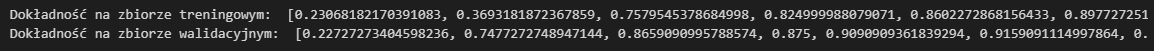
\includegraphics[width=15cm]{resources/model/images/scr-standard-result.png}
	\caption{Przykładowe wartości dokładności dla zbioru treningowe i walidacyjnego}
	\label{Fig:tests-wyniki-2}
\end{figure}
\FloatBarrier

\begin{figure}[ht]
	\centering
	\includegraphics[height=5.5cm]{resources/model/images/v2_epoch75.png}
	\caption{Przykładowa wizualizacja dokładności i straty wytrenowanego modelu}
	\label{Fig:tests-wyniki-1}
\end{figure}
\FloatBarrier

\subsubsection{Testy na danych zewnętrznych}
Po wyświetleniu dokładnosci modelu skrypt przeszukuje katalog z danymi i jego podkatalogi, by przygotować obrazy zewnętrzne.
Następnie ustawia ścieżkę do katalogu z obrazami testowymi i pobiera ich listę.
Dla każdego obrazu w tej liście wczytuje go, przeskalowuje do odpowiedniego rozmiaru i konwertuje do skali szarości
Następnie model przewiduje klasę obrazu, a wynik jest wyświetlany w konsoli.

\subsection{Testy modeli}
Model uczenia maszynowego jaki został wykorzystany w testach to sieć neuronowa.

Do testów stworzone zostało kilka modeli sieci neuronowych,
wytrenowanych na rysunkach grafów stworzonych za pomocą skryptów R.
Implementacja została wykonana biblioteką TensorFlow oraz Keras w języku Python.
Modele są w stanie rozpoznawać rysunki grafów i przypisywać im odpowiednie klasy.
Celem było również przetestowanie modeli na rzeczywistych zdjęciach,
zawierających wzorce przypominające grafy, bądź rysunkach grafów narysowanych ręcznie.

Stworzone zostały 3 modele:
- wytrenowany na danych ze stałą liczbą wierchołków
- wytrenowany na danych ze stałą liczbą wierchołków oraz walidacją krzyżową
- wytrenowany na danych ze zmienną liczbą wierzchołków

\subsection{Generacja danych}
Dane wygenerowane zostały przy pomocy skryptu stworzonego w języku R oraz biblioteki igraph.
Skrypt został zaprojektowany funkcyjnie, by osiągnąć możliwie największą automatyzację testów.
Rysunki grafów tworzone są o wielkości 800x600 pikseli, na białym tle, z wierzchołkami w kolorze pomarańczowym,
bez jakichkolwiek oznaczeń wierzchołków oraz zapisywane są w odpowiednich katalogach, odpowiadających klasie grafu.
Przygotowane zostały funkcje tworzące ścieżki, cykle, grafy pełne, grafy spójne, grafy dwudzielne oraz bezkrawędziowe.
W każdej z funkcji możliwy jest wybór liczby generowanych grafów, liczba wierzchołków grafu
oraz współczynnik odpowiadający za zakrzywienie krawędzi na rysunkach.

W testach wykorzystane zostały wszystkie typy grafów.
Każdy z nich, czyli dana liczba wierchołków i typ grafu, wygenerowany został w liczbie 500 sztuk
oraz ze stałą krzywizną krawędzi, wynoszącą 0,3. % Zastanowić się nad zmianą na losowe rozmieszczenie

\subsection{Dane zewnętrzne}
Obrazy testowe, które nazwane są tutaj danymi zewnętrznymi, są rysunkami grafów pochodzącymi spoza przygotowanego testu.
Dzielą się na obrazy pobrane z internetu, obrazy wygenerowane przez skrypt w R, ale nie używane w treningu
oraz rysunki odręczne grafów.

\subsection{Opis skryptu}

\subsubsection{Przygotowanie}
Skrypt rozpoczyna się od przygotowania środowiska do trenowania modelu.
Najpierw ustawia ścieżki do katalogów z wygenerowanymi grafami oraz do katalogów na dane treningowe i walidacyjne.
Następnie sprawdza, czy te katalogi istnieją, a jeśli nie, tworzy je.
Dalej, definiuje parametry dotyczące wielkości obrazów oraz wielkości partii danych, które będą używane podczas treningu.
Dla każdej wartości liczby wierzchołków ustawia ścieżkę do katalogu z wygenerowanymi grafami,
pobiera listę podkatalogów oraz obrazów w każdym z nich,
a następnie dzieli obrazy na zestawy treningowe i walidacyjne w stosunku 80:20.
Tworzy odpowiednie katalogi dla tych zestawów, jeśli jeszcze nie istnieją,
i kopiuje obrazy do właściwych lokalizacji, segregując je na treningowe i walidacyjne.

\subsubsection{Model}
Na początku dane zostały przygotowane ze zbioru obrazów, znajdującego się w katalogu lokalnym.
Dokonany został podział na zbiory treningowe i walidacyjne.
Dla każdego przejścia walidacji krzyżowej, dane zostały podzielone inaczej.
Po wczytaniu danych, zostały przeskalowane i przekształcone do odcieni szarości.

Model sieci neuronowej został zdefiniowany jako sekwencyjny stos warstw.
Pierwsza warstwa to warstwa Rescaling, która normalizuje wartości pikseli do zakresu [0, 1].
Następne trzy warstwy to Conv2D z wybraną liczbą filtrów, z których każda jest poprzedzona warstwą MaxPooling2D.
Warstwy konwolucyjne używają różnych funkcji akytwacji, np. ReLU.
Po warstwach konwolucyjnych znajduje się warstwa Flatten, która przekształca mapy cech 2D w wektor 1D.
Następnie dodana jest w pełni połączona (Dense) warstwa z wybraną liczbą jednostek
i wybraną funkcją aktywacji, wraz z warstwą dropout.
Zastosowana jest tam również regularyzacja L2 (zmniejszanie wag) z ustaloną siłą regularyzacji wynoszącą.
Warstwa wyjściowa zawiera tyle jednostek, ile występuje klas.
Zależnie od danego testu, może być to różna liczba.

Dla standaryzacji danego testu ustalono K-Fold z liczbą podziałów równą 5.
Dla wszystkich warstw wybrana została funkcja aktywacji ReLU.
Liczba epok wyniosła 75.
W przypadku warstw konwolucyjnych, wybrano 32 filtry, a dla warstwy w pełni połączonej zastosowano 128 jednostek.
Regularyzacja została zastosowana z siłą 0,01, a współczynnik dropout - 0,2.

\subsubsection{Wyniki}
Po wytrenowaniu modelu, skrypt wizualizuje dokładność i stratę modelu.
Najpierw wyświetla w konsoli wartości dokładności dla obu zbiorów z historii treningu.
Dalej tworzy wykresy, gdzie na pierwszym z nich pokazuje dokładność na zbiorze treningowym i walidacyjnym,
a na drugim wykresie prezentuje stratę modelu dla obu zbiorów.

\subsubsection{Testy na danych zewnętrznych}
Po wyświetleniu dokładnosci modelu skrypt przeszukuje katalog z danymi i jego podkatalogi, by przygotować obrazy zewnętrzne.
Następnie ustawia ścieżkę do katalogu z obrazami testowymi i pobiera ich listę.
Dla każdego obrazu w tej liście wczytuje go, przeskalowuje do odpowiedniego rozmiaru i konwertuje do skali szarości
Następnie model przewiduje klasę obrazu, a wynik jest wyświetlany w konsoli.

\subsection{Testy modeli}
\subsubsection{Model podstawowy}

\begin{figure}[ht]
	\centering
	\includegraphics[height=5.5cm]{partials/images/tests/v2_epoch75.png}
	\caption{Wyniki testów dla modelu podstawowego}
\label{Fig:GraphUndirected}
\end{figure}
\FloatBarrier

\begin{figure}[ht]
	\centering
	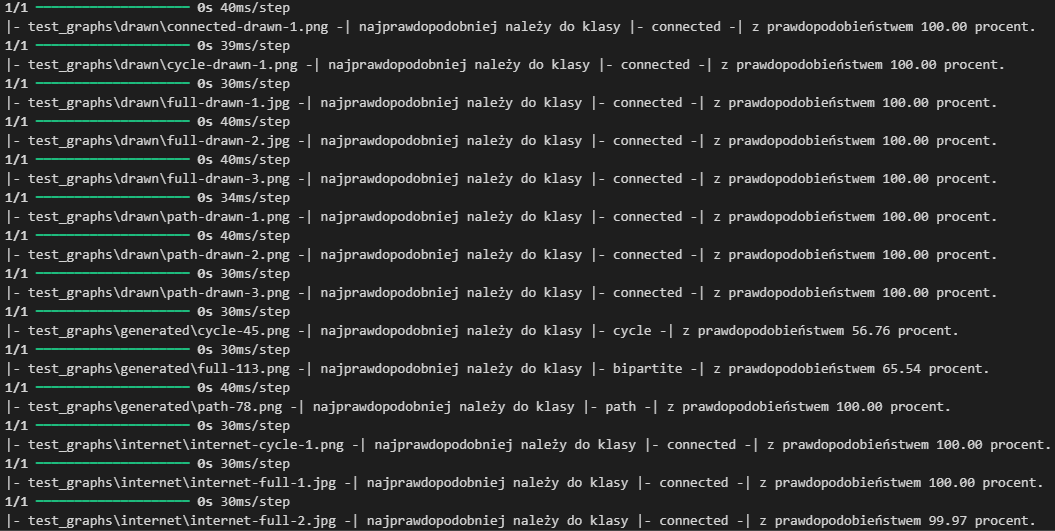
\includegraphics[height=7cm]{partials/images/tests/v2_epoch75_img_tests.png}
	\caption{Klasyfikacja obrazów zewnętrznych dla modelu ze zmienną liczbą wierzchołków}
\label{Fig:GraphUndirected}
\end{figure}
\FloatBarrier

\subsubsection{Model z walidacją krzyżową}

W przypadku standardowego modelu z walidacją krzyżową model bardzo szybko uległ przeuczeniu.
Już po szóstej iteracji dokładność na zbiorze walidaycjnym wyniosła 100\%, co nie jest realistycznie możliwe.
Została podjęta próba ograniczenia przeuczenia poprzez zwiększenie zbioru danych, zmiany liczby epok w modelu
oraz manipulacji współczynnikami dropout i regularyzacji.
W każdym przypadku model zwracał niezadowalające wyniki wynoszące 100\% po jednej z początkowych iteracji.

\begin{figure}[ht]
	\centering
	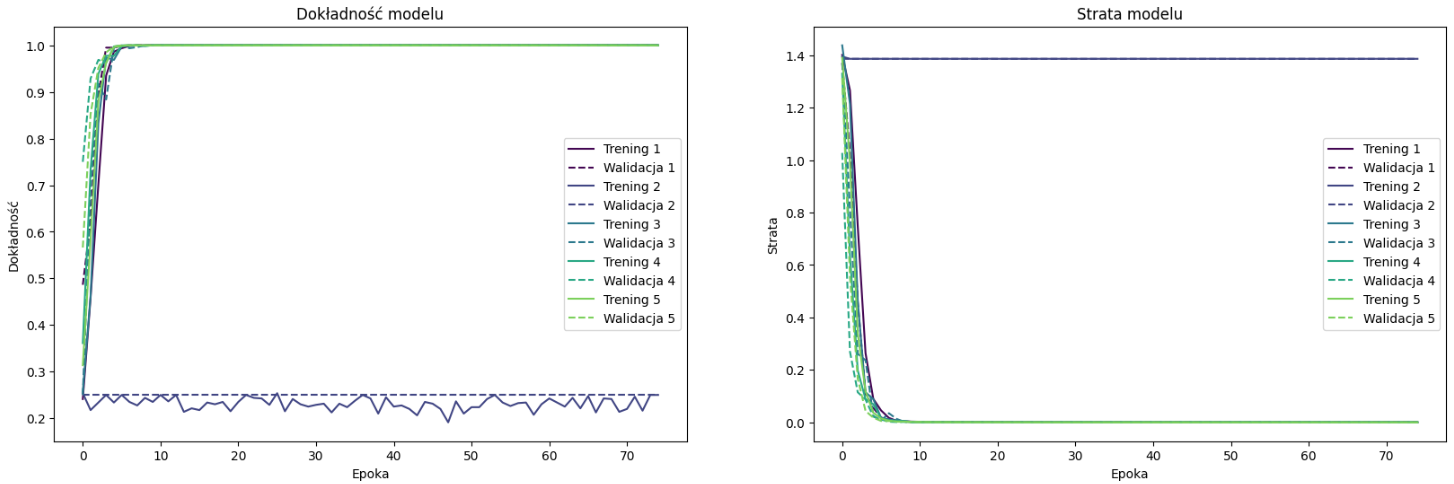
\includegraphics[height=5.5cm]{partials/images/tests/v2_crossvalid.png}
	\caption{Wyniki testów dla modelu z walidacją krzyżową}
\label{Fig:GraphUndirected}
\end{figure}
\FloatBarrier

Z powodu przeuczenia model nie radził sobie z zewnętrznymi obrazkami testowymi.
Większość grafów określił jako grafy pełne, co nie jest zgodne ze stanem rzeczywistym.

\begin{figure}[ht]
	\centering
	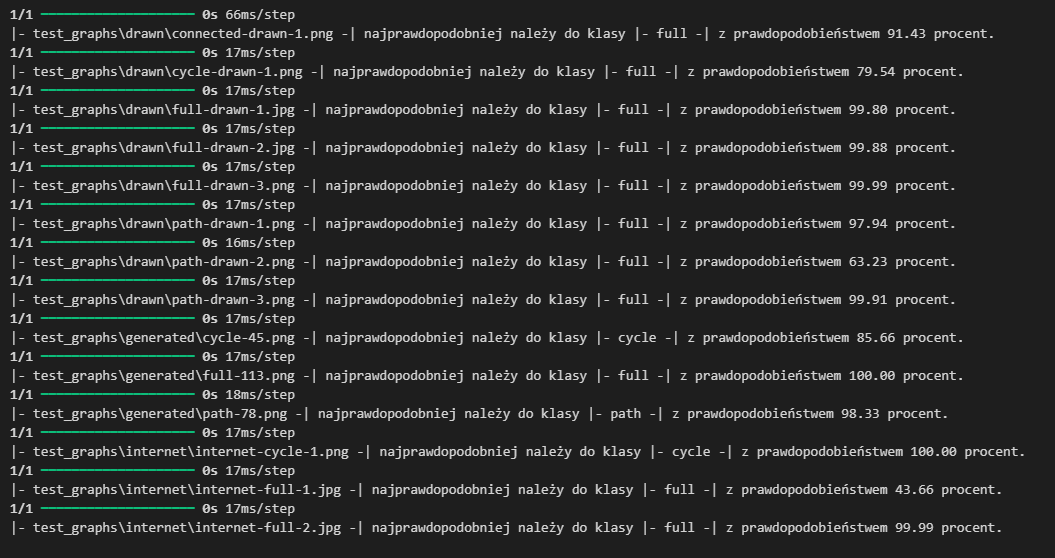
\includegraphics[height=7cm]{partials/images/tests/v2_crossvalid_img_tests.png}
	\caption{Klasyfikacja obrazów zewnętrznych dla modelu z walidacją krzyżową}
\label{Fig:GraphUndirected}
\end{figure}
\FloatBarrier

\subsubsection{Model ze zmienną liczbą wierzchołków}
Najlepsze wyniki pod względem rozpoznawania zewnętrznych obrazków testowych
oraz realistycznej dokładności na zbiorze walidacyjnym,
zostały uzyskane przy użyciu modelu sieci neuronowej uczonej na rysunkach grafów z różną liczbą wierzchołków.
Było to odpowiednio 4, 5, 6 oraz 7 wierzchołków.

\begin{figure}[ht]
	\centering
	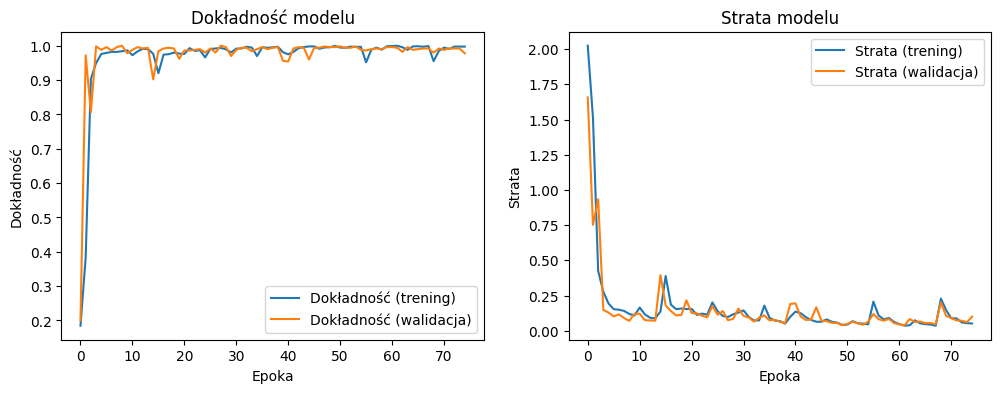
\includegraphics[height=5.5cm]{partials/images/tests/v2_multiple_edges_epoch75.png}
	\caption{Wyniki testów dla modelu ze zmienną liczbą wierzchołków}
\label{Fig:GraphUndirected}
\end{figure}
\FloatBarrier

Model nie poradził sobie zbyt dobrze z obrazami zewnętrznymi, lecz znacznie lepiej niż model z walidacją krzyżową.
Poprawnie wskazanych klas grafów było 5 z 14 wszystkich rysunków.
Mimo, że model jest w stanie poprawnie określić niektóre typy grafów poprawnie,
wciąż jest to dokładność niższa niż 50\%.

\begin{figure}[ht]
	\centering
	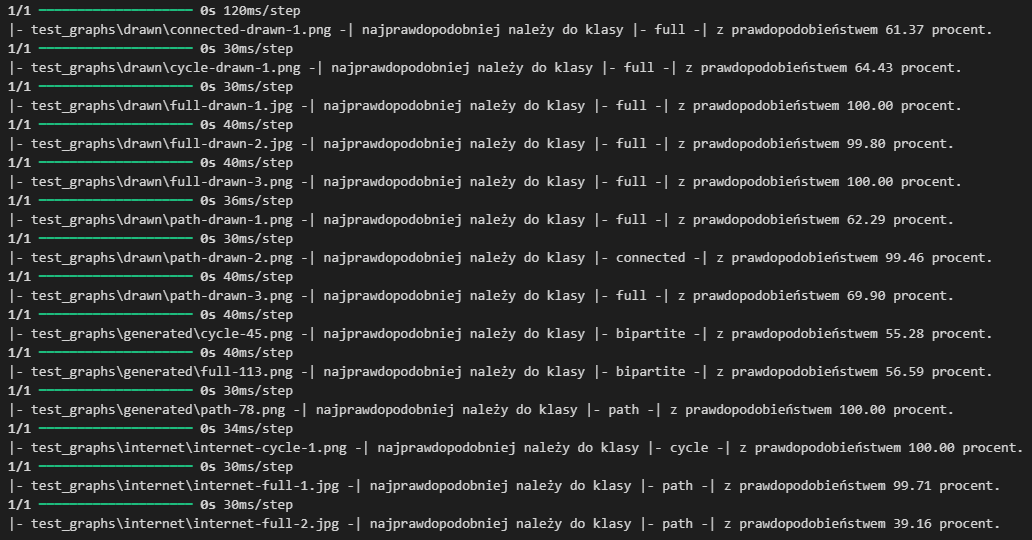
\includegraphics[height=7cm]{partials/images/tests/v2_multiple_edges_epoch75_img_tests.png}
	\caption{Klasyfikacja obrazów zewnętrznych dla modelu z walidacją krzyżową}
\label{Fig:GraphUndirected}
\end{figure}
\FloatBarrier

\subsubsection{Model ze zmienną liczbą wierzchołków i walidacją krzyżową}

\begin{figure}[ht]
	\centering
	% \includegraphics[height=5.5cm]{partials/images/tests/v2_multiple_edges_crossvalid.png}
	\caption{Wyniki testów dla modelu ze zmienną liczbą wierzchołków i walidacją krzyżową}
\label{Fig:GraphUndirected}
\end{figure}
\FloatBarrier

\begin{figure}[ht]
	\centering
	% \includegraphics[height=5.5cm]{partials/images/tests/v2_multiple_edges_crossvalid_img_tests.png}
	\caption{Klasyfikacja obrazów zewnętrznych dla modelu ze zmienną liczbą wierzchołków i walidacją krzyżową}
\label{Fig:GraphUndirected}
\end{figure}
\FloatBarrier

\subsection{Wnioski}
W przypadku uczenia modeli z wykorzystaniem grafów pełnych, najczęściej dominowały one cały zbiór danych,
przez co modele w kolejnych testach klasyfikowały większość testowych grafów rysowanych odręcznie jako właśnie grafy pełne.

Testy z wykorzystaniem stałej liczby wierzchołków grafów okazały się mniej owocne niż testy z rysunkami grafów
o zmiennej liczbie wierchołków.

Wystąpiła tendencja do niepoprawnego określania innych grafów, grafami dwudzielnymi, jeśli takie znajdowały się
w zbiorze danych uczących.

\subsection{Wnioski}
% -- TO DO -- %
W testach zastosowano naukę na maksymalnie 75 epokach.
Analizując krzywe dokładności i straty modeli, można dojść do wniosku,
że dłuższe uczenie nie przyniosłoby pozytywnych skutków lub znikome pozytywne.
Przeprowadzono również testy na mniejszych liczbach epok, lecz wartości takie jak 10, czy 20,
są za małe, by poprawnie nauczyć większość modeli.
Modeli osiągały dość wysokie dokładności już po kilku pierwszych epokach,
ale zdecydowana większość z nich, z biegiem kolejnych epok, nabierała jeszcze lepszej dokładności.

W przypadku jednego modelu, konieczne było zmniejszenie liczby epok do 55,
ze względu na powstające problemy z procesem nauczania, po owej epoce.

Uczenie modeli z wykorzystaniem stałej liczby wierzchołków grafów okazało się bardziej skuteczne
niż nauka na rysunkach grafów o zmiennej liczbie wierzchołków.

Skomplikowaność modelu i zastosowane techniki optymalizacyjne rzadko przekładały się na zwiększoną realną dokładność modelu.

W przypadku uczenia najbardziej zmodyfikowanych modeli, to grafy pełne najczęściej dominowały cały zbiór danych,
przez co modele te testach na danych zewnętrznych,
klasyfikowały większość testowych grafów rysowanych odręcznie jako właśnie grafy pełne.